\section{Problem definition}

\begin{frame}[plain]
   \sectionpage
\end{frame}

\begin{frame}
   \frametitle{Home care in Brazil}

   \textbf{Motivation: } Solve a real problem in Porto Alegre

   \vspace{12pt}

   \textbf{Pilot program ``Better in Home''}
   \begin{itemize}
      \item Provider of home hospitalization
      \item Motivation: population growth and aging
      \item Opportunity for \textbf{knowledge transfer}
      \item Current approach: manual planning
   \end{itemize}

   \begin{tikzpicture}[overlay]
      \node (a) at (11.6,2) {
         
\includegraphics[scale=0.2]{fig/melhor-em-casa.png}
      };
      \node [below=1pt of a] {Source: DATASUS (2021)};
   \end{tikzpicture}
\end{frame}

\begin{frame}
   \frametitle{Home care in Brazil}

   \textbf{Pilot program ``Better in Home''}
   \begin{itemize}
      \item Program started in 2016
      \item Experimental on some big Brazilian cities
      \item Target population: patients eligible to home hospitalization
   \end{itemize}

   \begin{tikzpicture}[overlay]
   \node (a) at (12.2,0) {
      
\includegraphics[scale=0.2]{fig/melhor-em-casa.png}
   };
   \node [below=1pt of a] {Source: DATASUS (2021)};
   \end{tikzpicture}

\end{frame}

\begin{frame}
   \frametitle{Home Care in Porto Alegre}

   \textbf{Current problem and solution approach}
   \begin{itemize}
      \item 19 ``teams''
      \item 300 patients per week
      \item Most of the \textbf{planning is manual}, daily basis
      \item One experienced caregiver
   \end{itemize}


\end{frame}

\begin{frame}
   \frametitle{Home Care in Porto Alegre}


   \textbf{Three-step manual approach}
   \begin{itemize}
      \item Step 1: chooses the patient of the day
      \item Step 2: assign the patients to the teams
      \item Step 3: individual routing of the teams
      \begin{itemize}
         \item Done by the vehicle drive
         \item Mostly a ``nearest neighbor'' strategy
      \end{itemize}
      \item ``Hope for the best'' strategy
   \end{itemize}

\end{frame}

\begin{frame}
   \frametitle{Home Care in Porto Alegre}

   \vspace*{8pt}

   \textbf{Currently solved manually}
   \begin{itemize}
      \item Patient demands are set weekly
      \item The (manual) planning done daily
      \item First step: choice of patients of the day
      \item Second step: patient-team assignment
      \item Third step: individual routing by each team
   \end{itemize}

\end{frame}

\begin{frame}
   \frametitle{Home Care in Porto Alegre}

   \textbf{The problem is much more complex}
   \begin{itemize}
      \item Uncertainty regarding patients $\Rightarrow$ re-scheduling
      \item Less vehicles available than the number of teams
      \item Equipment needs to be carried according teams's planning
      \item Selection of training medical student
   \end{itemize}
\end{frame}

\begin{frame}
   \frametitle{Choosing a target problem}

   \textbf{Our methodology}
   \begin{itemize}
      \item Find, or propose a \textit{core} optimization problem
      \item Complex enough
      \begin{itemize}
         \item Valuable for the practitioner
         \item Interesting from the scientific perspective
      \end{itemize}
      \item But not too much constrained/specific
   \end{itemize}

   \vspace*{18pt}
  \pause


   \textbf{Problem of choice: } The Home Health Care Routing \\
   \qquad \qquad \qquad \qquad ~~~~ and Scheduling Problem (HHCRSP)


   \begin{tikzpicture}[overlay]
   \node (a) at (11.8,3) {
      
\includegraphics[scale=0.13]{fig/mankowska2014-paper.png}
   };
   \node [below=1pt of a] {\footnotesize \citet{mankowska2014}};
   \end{tikzpicture}

\end{frame}

\begin{frame}
   \frametitle{Our target problem}

   \textbf{The home health care routing and scheduling problem}
   \begin{itemize}
      \item HHCRSP was introduced by \citet{mankowska2014}
      \item Routing (caregivers) and scheduling (visit time)
      \item A model, and heuristics
      \item A public standard benchmark dataset
   \end{itemize}

%   \vspace{20pt}

%   \centering\includegraphics[width=0.9\textwidth]{img/skilled}

\end{frame}

\begin{frame}
   \frametitle{Our target problem}

   \textbf{On future interactions with HC managers}
   \begin{itemize}
      \item Uncertainty regarding attendance times
      \item Last minute changes on the availability of patients
      \item Current bottleneck: lack of infrastructure to interact with optimization algorithms
      \item Export the algorithms and processes to other Brazilian cities
   \end{itemize}
\end{frame}

\frame{
   \frametitle{The HHCRSP}

   \textbf{Main characteristics}
   \begin{enumerate}
      \item Routing components
      \item Patient time-window
      \item Covered service types
      \item Operations synchronization on multiple visits
   \end{enumerate}
}

\frame{
   \frametitle{The HHCRSP}

   \textbf{Main characteristics}
   \begin{enumerate}
      \item \textcolor{InfRed}{Routing components}
      \item Patient time-window
      \item Covered service types
      \item Operations synchronization on multiple visits
   \end{enumerate}
}

\frame{
   \frametitle{The HHCRSP: Routing features}
   \textbf{Routing components}
   \begin{itemize}
      \item Single transportation mode
      \item Routes start and finish at the depot
      \item Travel time between locations
      \item All visits must be performed
   \end{itemize}

%   \vspace*{12pt}

   \begin{figure}
      \includegraphics[width=0.7\textwidth,page=7]{fig/routing-example}
   \end{figure}
}

\frame{
   \frametitle{The HHCRSP}

   \textbf{Main characteristics}
   \begin{enumerate}
      \item \onlyh{1}{InfRed}{Routing components}
      \item \onlyh{2}{InfRed}{Patient time-window}
      \item Covered service types
      \item Operations synchronization on multiple visits
   \end{enumerate}
}

\frame{
   \frametitle{The HHCRSP: Routing features}
   \textbf{Soft time-window}
   \begin{itemize}
      \item Each patient/node has a time-window
      \item ``Hard'' time-window start
      \item ``Soft'' time-window ending
      \item Violated time-window ending: incurs additional cost
   \end{itemize}

   \begin{figure}[H]
      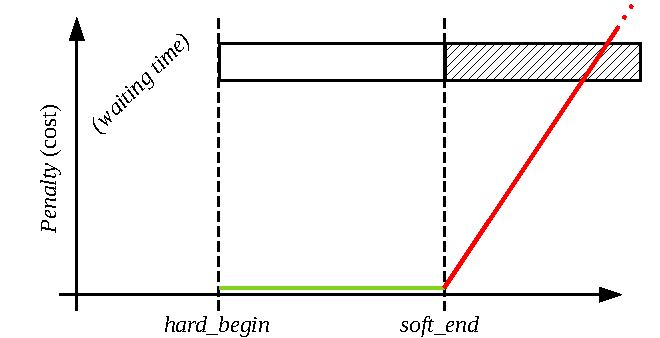
\includegraphics[width=0.6\textwidth]{fig/tw-penal.pdf}
   \end{figure}
}

\frame{
   \frametitle{The HHCRSP}

   \textbf{Main characteristics}
   \begin{enumerate}
      \item Routing components
      \item \onlyh{1}{InfRed}{Patient time-window}
      \item \onlyh{2}{InfRed}{Covered service types}
      \item Operations synchronization on multiple visits
   \end{enumerate}
}

\frame{
   \frametitle{The HHCRSP: domain features}

   \textbf{Covered service types}
   \begin{itemize}
      \item Set $\Sk$ of offered services
      \item A patient can require \textit{one}, or \textit{two services}
      \item Each service requested has a \textit{processing time}
      \item Caregivers have \textit{qualification} to perform only a few service types
   \end{itemize}

   \vspace*{8pt}

    \begin{figure}[H]
      \includegraphics[width=0.9\textwidth]{fig/skilled}
   \end{figure}

}

\frame{
   \frametitle{The HHCRSP}

   \textbf{Main characteristics}
   \begin{enumerate}
      \item Routing components
      \item Patient time-window
      \item \onlyh{1}{InfRed}{Covered service types}
      \item \onlyh{2}{InfRed}{Operations synchronization on multiple visits}
   \end{enumerate}
}


\begin{frame}
   \frametitle{The HHCRSP: domain features}
   \textbf{Operations synchronization on double service patients}
   \begin{itemize}
      \item Special requirement for patients requiring two service types
      \item Services must start simultaneously in some patients
      \item Others have precedence constraints
      \item Common feature container allocation/transshipment problems \citep{drexl2012synchronization}
   \end{itemize}

%   \vspace*{8pt}

   \begin{figure}[H]
      \includegraphics[width=1\textwidth,page=2]{fig/skilled}
   \end{figure}

\end{frame}

\begin{frame}
   \frametitle{The HHCRSP: Own characteristics}
   \textbf{Double service: precedence order}
   \begin{itemize}
      \item Service precedence: 2 > 5
      \item ($\delta^\mathrm{min}$) and ($\delta^\mathrm{max}$): separation time
   \end{itemize}

   \begin{figure}
      \centering
      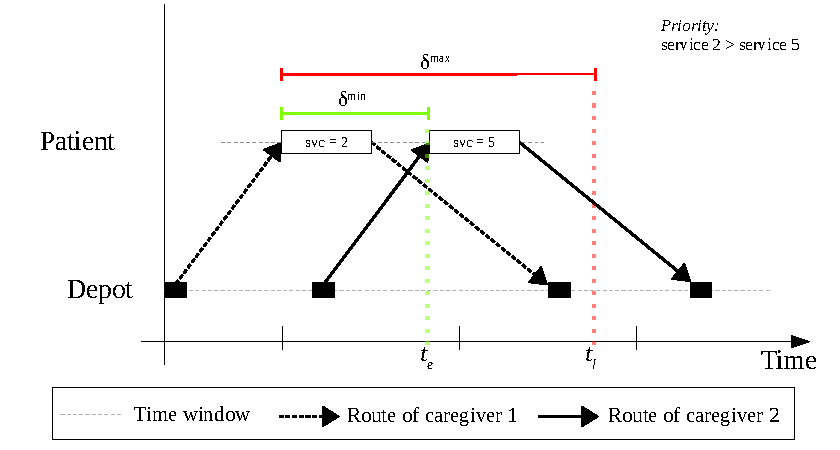
\includegraphics[width=0.6\textwidth,page=1]{fig/sync-tsn2}
   \end{figure}
\end{frame}

\begin{frame}
   \frametitle{The HHCRSP: Own characteristics}
   \textbf{Double service: parallel attendance}
   \begin{itemize}
      \item Services must start simultaneously
   \end{itemize}

   \begin{figure}
      \centering
      \includegraphics[width=0.6\textwidth,page=2]{fig/sync-tsn2}
   \end{figure}
\end{frame}

\begin{frame}
   \frametitle{The HHCRSP: some formal definitions}
   \textbf{Main sets}
   \begin{itemize}
      \item $\mathcal{V}$ : Vehicles/caregivers
      \item $\mathcal{C}$ : Patients/nodes
      \item $\mathcal{S}$ : Service types/skills
   \end{itemize}

\end{frame}

\frame{
   \frametitle{The HHCRSP: some formal definitions}

   \textbf{Objective function}

   \only<1> {
      \begin{gather}
         \mathrm{Minimize~} \lambda_1 D \; +
         \lambda_2 T \; +
         \lambda_3 T^\mathit{max} \nonumber
      \end{gather}
   }

   \only<2> {
      \begin{gather}
      \mathrm{Minimize~}\color{InfRed} \lambda_1 \normalcolor D \; +
      \color{green} \lambda_2 \normalcolor T \; +
      \color{blue} \lambda_3 \normalcolor T^\mathit{max} \nonumber
      \end{gather}
   }

   \vspace*{12pt}

   \textbf{Components}
   \begin{itemize}
      \item $D$: Sum of traveled distance
      \item $T$: Sum of tardiness
      \item $T^\mathrm{max}$: Maximum tardiness
   \end{itemize}

%   \begin{tikzpicture}[overlay]
%      \draw<3>[InfRed,line width=2pt] (4.3,3.4) rectangle +(0.9, 0.7);
%      \draw<3>[InfRed,line width=2pt] (-0.4, 1.54) rectangle +(6.4, 0.7);
%      \draw<4>[InfRed,line width=2pt] (5.55,3.4) rectangle +(0.9, 0.7);
%      \draw<4>[InfRed,line width=2pt] (-0.4, 0.95) rectangle +(6.4, 0.7);
%      \draw<5>[InfRed,line width=2pt] (6.85, 3.4) rectangle +(1.3, 0.7);
%      \draw<5>[InfRed,line width=2pt] (-0.4, 0.35) rectangle +(6.4, 0.7);
%   \end{tikzpicture}
}